\chapter{Referencial Teórico}
\label{cap:referencial-teorico}

Neste capítulo serão apresentados os assuntos considerados fundamentais para o entendimento dos processos que estão envolvidos no uso das tecnologias abordadas no decorrer do trabalho. No início será discutida a criação dos shaders e seu uso ao longo do tempo, em seguida serão expostos itens de ordem técnica sobre os shaders e os motores de jogo. Ao final será tratada a integração dessas tecnologias com os processos de otimização.

\section{História da Evolução da Programação de Shaders}
\label{sec:historia-evolucao-programacao-shaders}

As representações visuais feitas através de imagens foram e são até hoje uma característica importante da formação da humanidade. Através do sentido da visão conseguimos absorver informações rapidamente, fazer associações durante o aprendizado e o estudo, ou ainda distinguir se algo é visualmente agradável o suficiente ou não para prender nossa atenção. O caso mais extremo seria a discussão da existência de algo que não se pode ver, como no século dezessete, quando a existência das bactérias era muito questionada, até que Antonie van Leeuwenhoek inventou o microscópio (LUTEN, 2014)\nocite{openGLBook}.

Bem no início do desenvolvimento dos primeiros computadores, quando seu acesso era destinado a um público mais restrito devido aos custos elevados e a logística complexa, a forma de representação visual para os humanos dos pulsos elétricos gerados pelo processamento de dados nos computadores era feita através de várias lâmpadas conectadas em placas ou de cartões de papel perfurados (um processo que, em alguns casos, poderia demorar várias horas para terminar). Esse cenário só começou a mudar depois da aplicação da tecnologia do tubo de raios catódicos (\acrshort{CRT}), em 1951, pelo MIT (\acrlong{MIT}) para visualizar a saída de um programa de computador instantaneamente. Cabe ainda ressaltar que a partir de então ele continuou sendo usado até o advento das novas tecnologias de monitores e televisores de tela plana (LUTEN, 2014)\nocite{openGLBook}.

Apesar do avanço citado acima, o estabelecimento da computação gráfica como conhecemos hoje teve início apenas 10 anos depois. A partir da criação de um programa de computador por Ivan Sutherland chamado Sketchpad, que permitia que o usuário desenhasse formas geométricas utilizando uma caneta óptica em um \acrshort{CRT} que permitia a visualização em tempo real (LUTEN, 2014)\nocite{openGLBook}. Isso causou uma mudança de padrão na forma como as pessoas entendiam e utilizavam os computadores e foi o ponto de partida para o estudo e desenvolvimento da computação gráfica em tempo real e também das interfaces gráficas de usuário (\acrshort{GUI}).

	\begin{figure}[h!]
		\centering
		\Caption{\label{fig:exemplo-1} Demonstração do programa de computador Sketchpad}	
		\UNIFORfig{}{
			\fbox{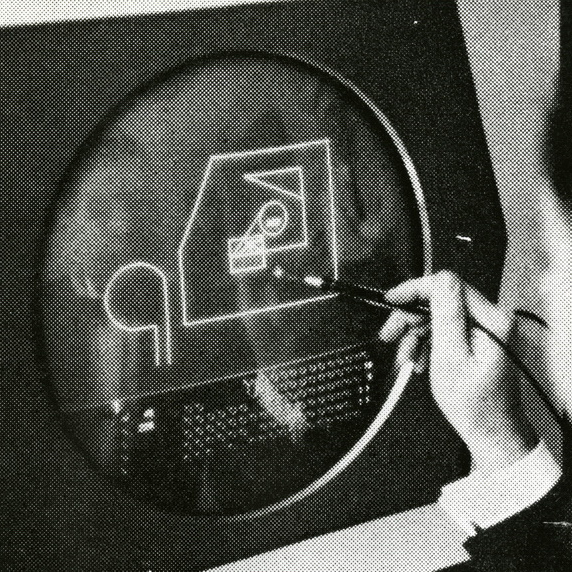
\includegraphics[width=8cm]{figuras/figura-1}}
		}{
			\Fonte{http://i0.wp.com/www.designleap.org/wp-content/uploads/2014/06/Sketchpad-Ivan-Sutherland-1963.jpg?resize=572\%2C572}
		}	
	\end{figure}
	\nocite{figura1}
	
Com o avanço resultado da criação dos circuitos integrados, cujo uso nos microprocessadores proporcionou um espantoso crescimento da indústria, os computadores deixaram de ser um monopólio das grandes companhias e tornaram-se muito mais acessíveis a pessoas simples. Isso abriu várias possibilidades para o mercado de computadores pessoais, entre elas destaca-se o surgimento das primeiras placas gráficas produzidas pela IBM (\acrlong{IBM}).

    \begin{figure}[h!]
		\centering
		\Caption{\label{fig:exemplo-2} Placa gráfica denominada Color Graphics Adapter produzida nos anos 80 pela IBM.}	
		\UNIFORfig{}{
			\fbox{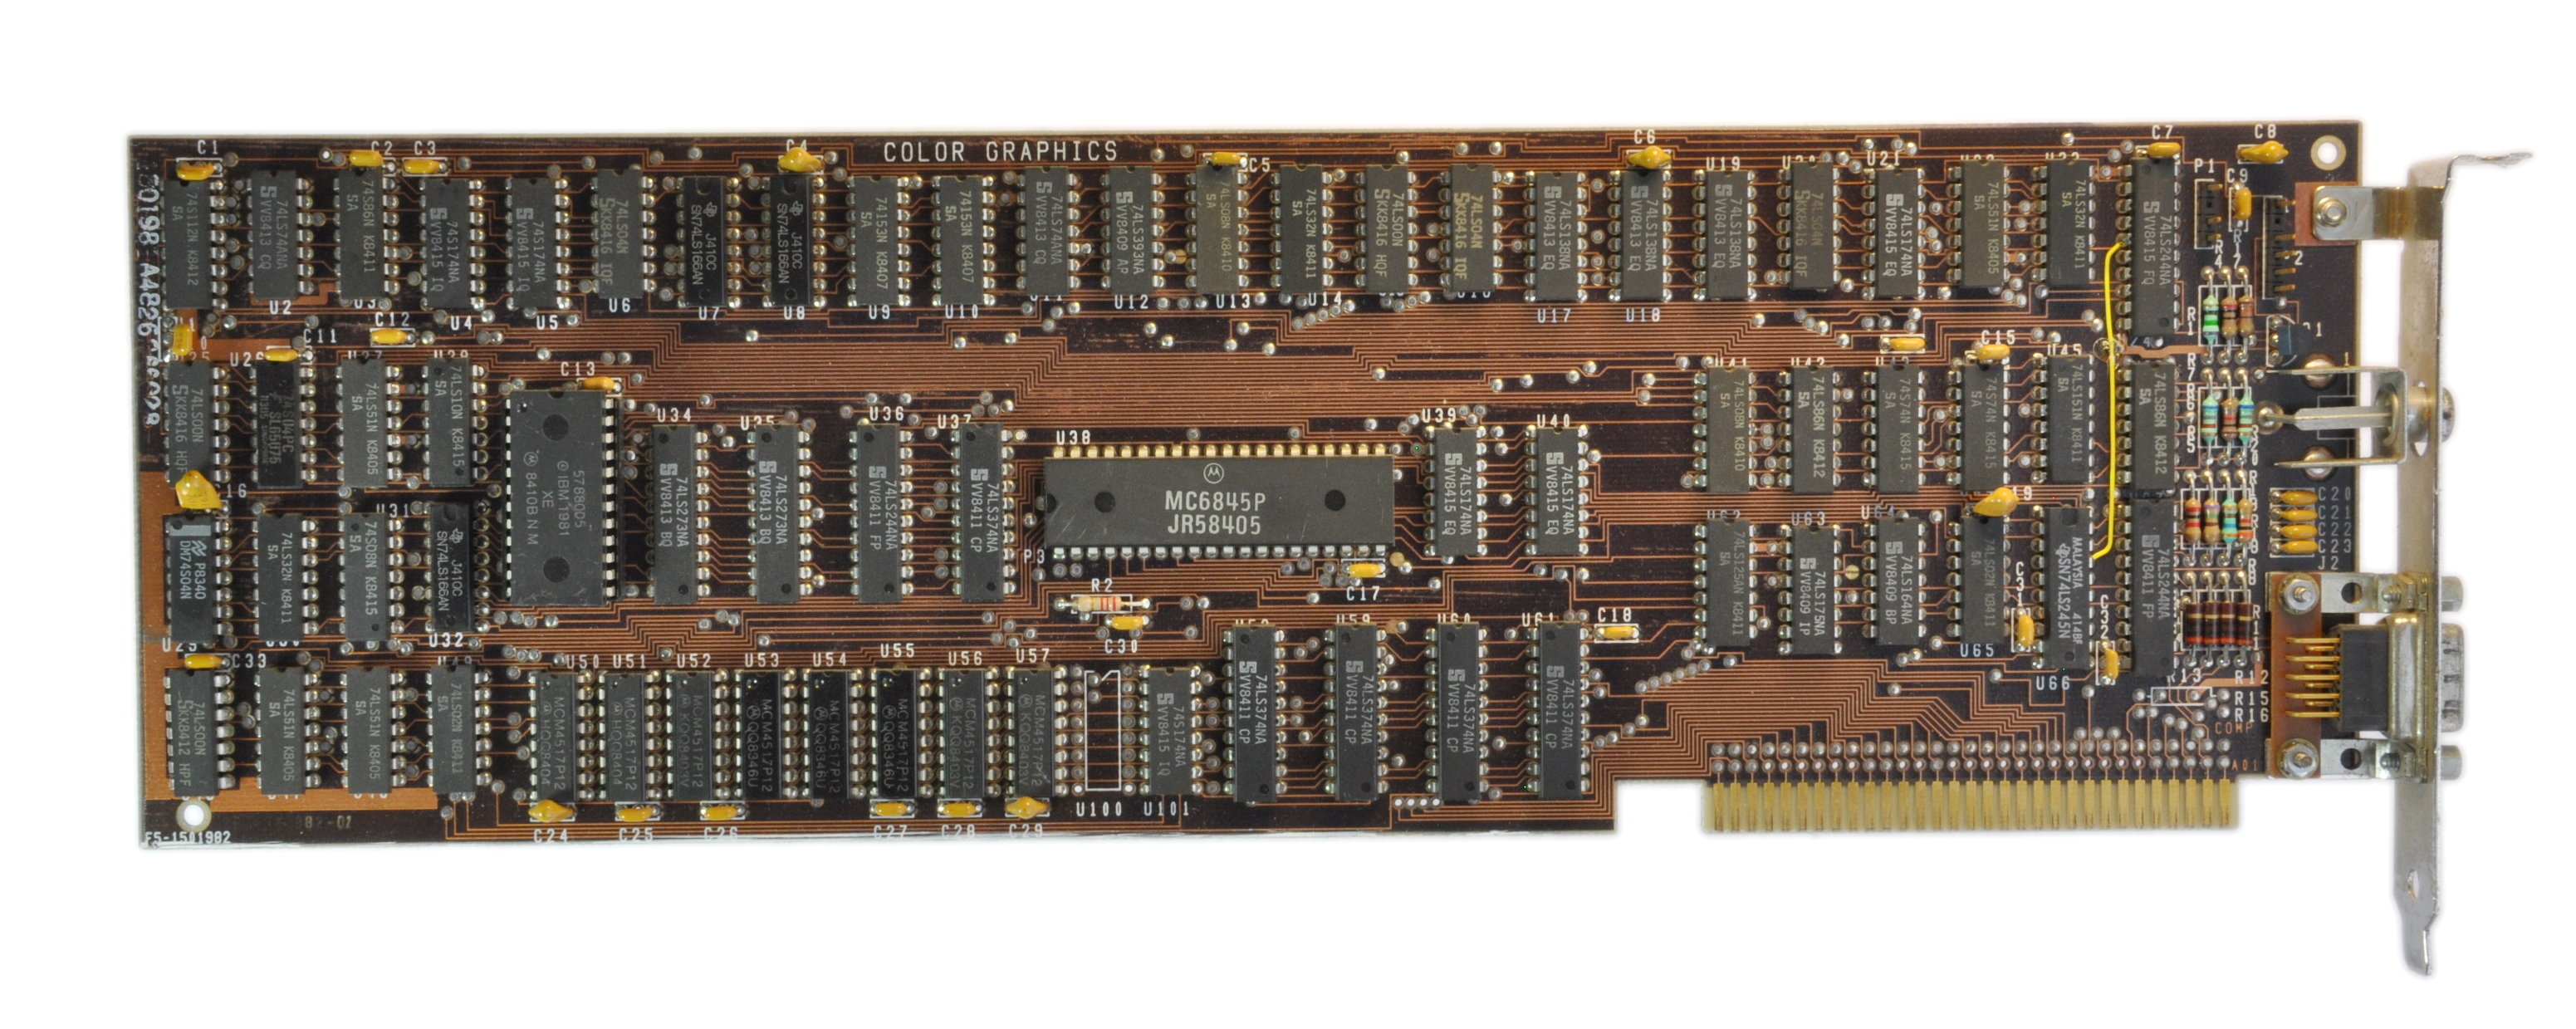
\includegraphics[width=15cm]{figuras/figura-2}}
		}{
			\Fonte{https://upload.wikimedia.org/wikipedia/commons/5/55/IBM\_Color\_Graphics\_Adapter.jpg}
		}	
	\end{figure}
	\nocite{figura2}
	
Como a indústria de jogos eletrônicos tinha mais recursos para explorar devido às melhorias de hardware disponíveis, vários jogos começaram a se destacar no mercado. Entre eles os mais marcantes para a popularização do uso de tecnologia de computação gráfica tridimensional foram lançados pela empresa id Software na década de 90. O primeiro sendo Wolfenstein 3D (que na realidade utilizava o modo 7 do Super NES (\acrlong{NES}) para emular a ambientação tridimensional) que definiu o padrão para jogos no gênero de tiro em primeira pessoa em 3D e o segundo sendo Doom que fazia uso de renderização com perspectiva 3D em tempo real por meio de software proprietário desenvolvido pela própria id Software voltado para produção com destino a computadores que utilizavam o sistema operacional da Microsoft (\acrshort{MS-DOS}).

    \begin{figure}[h!]
		\centering
		\Caption{\label{fig:exemplo-3} No lado esquerdo percebe-se que Doom fazia uso de 3D real enquanto no lado direito Wolfenstein posicionava imagens 2D em diferentes camadas para simular a profundidade tridimensional.}	
		\UNIFORfig{}{
			\fbox{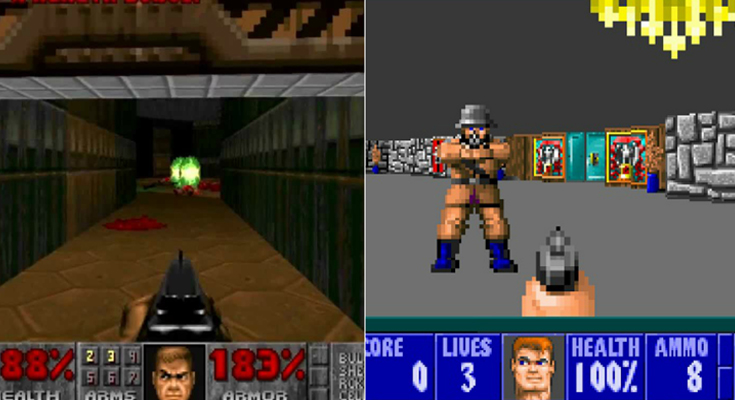
\includegraphics[width=13cm]{figuras/figura-3}}
		}{
			\Fonte{https://www.retrorefurbs.com/wolfenstein-vs-doom-the-battle-of-the-first-person-shooters/}
		}
	\end{figure}
	\nocite{figura3}
	
Paralelo ao cenário desses jogos (LUTEN, 2014)\nocite{openGLBook}, a Silicon Graphics (\acrshort{SGI}), uma companhia especializada em computação gráfica 3D e líder de mercado na época, trabalhava no lançamento open source da Open Graphics Library (\acrshort{OpenGL}), uma API (\acrlong{API}) padronizada multiplataforma de processamento de gráficos de computador em tempo real que rapidamente dominou o mercado, e que era uma derivação de outra biblioteca proprietária da mesma empresa, a IRIS GL (\acrlong{IRIS GL}). 

Vendo uma oportunidade de mercado, a Microsoft logo agiu e comprou a empresa RenderMorphics, criadora da \acrshort{API} Reality Lab, que teve o nome alterado para Direct3D e foi distribuido como um SDK (\acrlong{SDK}) conhecido como DirectX (LUTEN, 2014)\nocite{openGLBook}, acabando por se tornar o concorrente direto da \acrshort{OpenGL}. Essa rivalidade no final das contas acabou sendo benéfica tanto para o mercado de jogos eletrônicos quanto para os seus consumidores, já que acelerou o desenvolvimento de novas tecnologias que exploravam ao máximo o potencial do hardware disponível.
	
Mais adiante, em 1999, a empresa NVIDIA foi responsável for trazer mais uma inovação ao mercado, a "primeira GPU" (\acrlong{GPU}) foi como ficou conhecida a placa gráfica GeForce 256 (Figura 4), que fazia uso de uma tecnologia chamada T\&L (\acrlong{T+L}) que basicamente movia os cálculos de transformação e iluminação de vértices da CPU (\acrlong{CPU}) para a \acrshort{GPU}. Isso permitia uma maior velocidade em operações matemáticas de ponto flutuante. Então nos próximos anos o que se viu foi um crescimento exponencial de performance de \acrshort{GPU} para renderização em tempo real.

    \begin{figure}[h!]
		\centering
        \Caption{\label{fig:1} Hardware da placa gráfica da NVIDIA.}
        \begin{subfigure}{0.50\textwidth}
        \UNIFORfig{}{
			\fbox{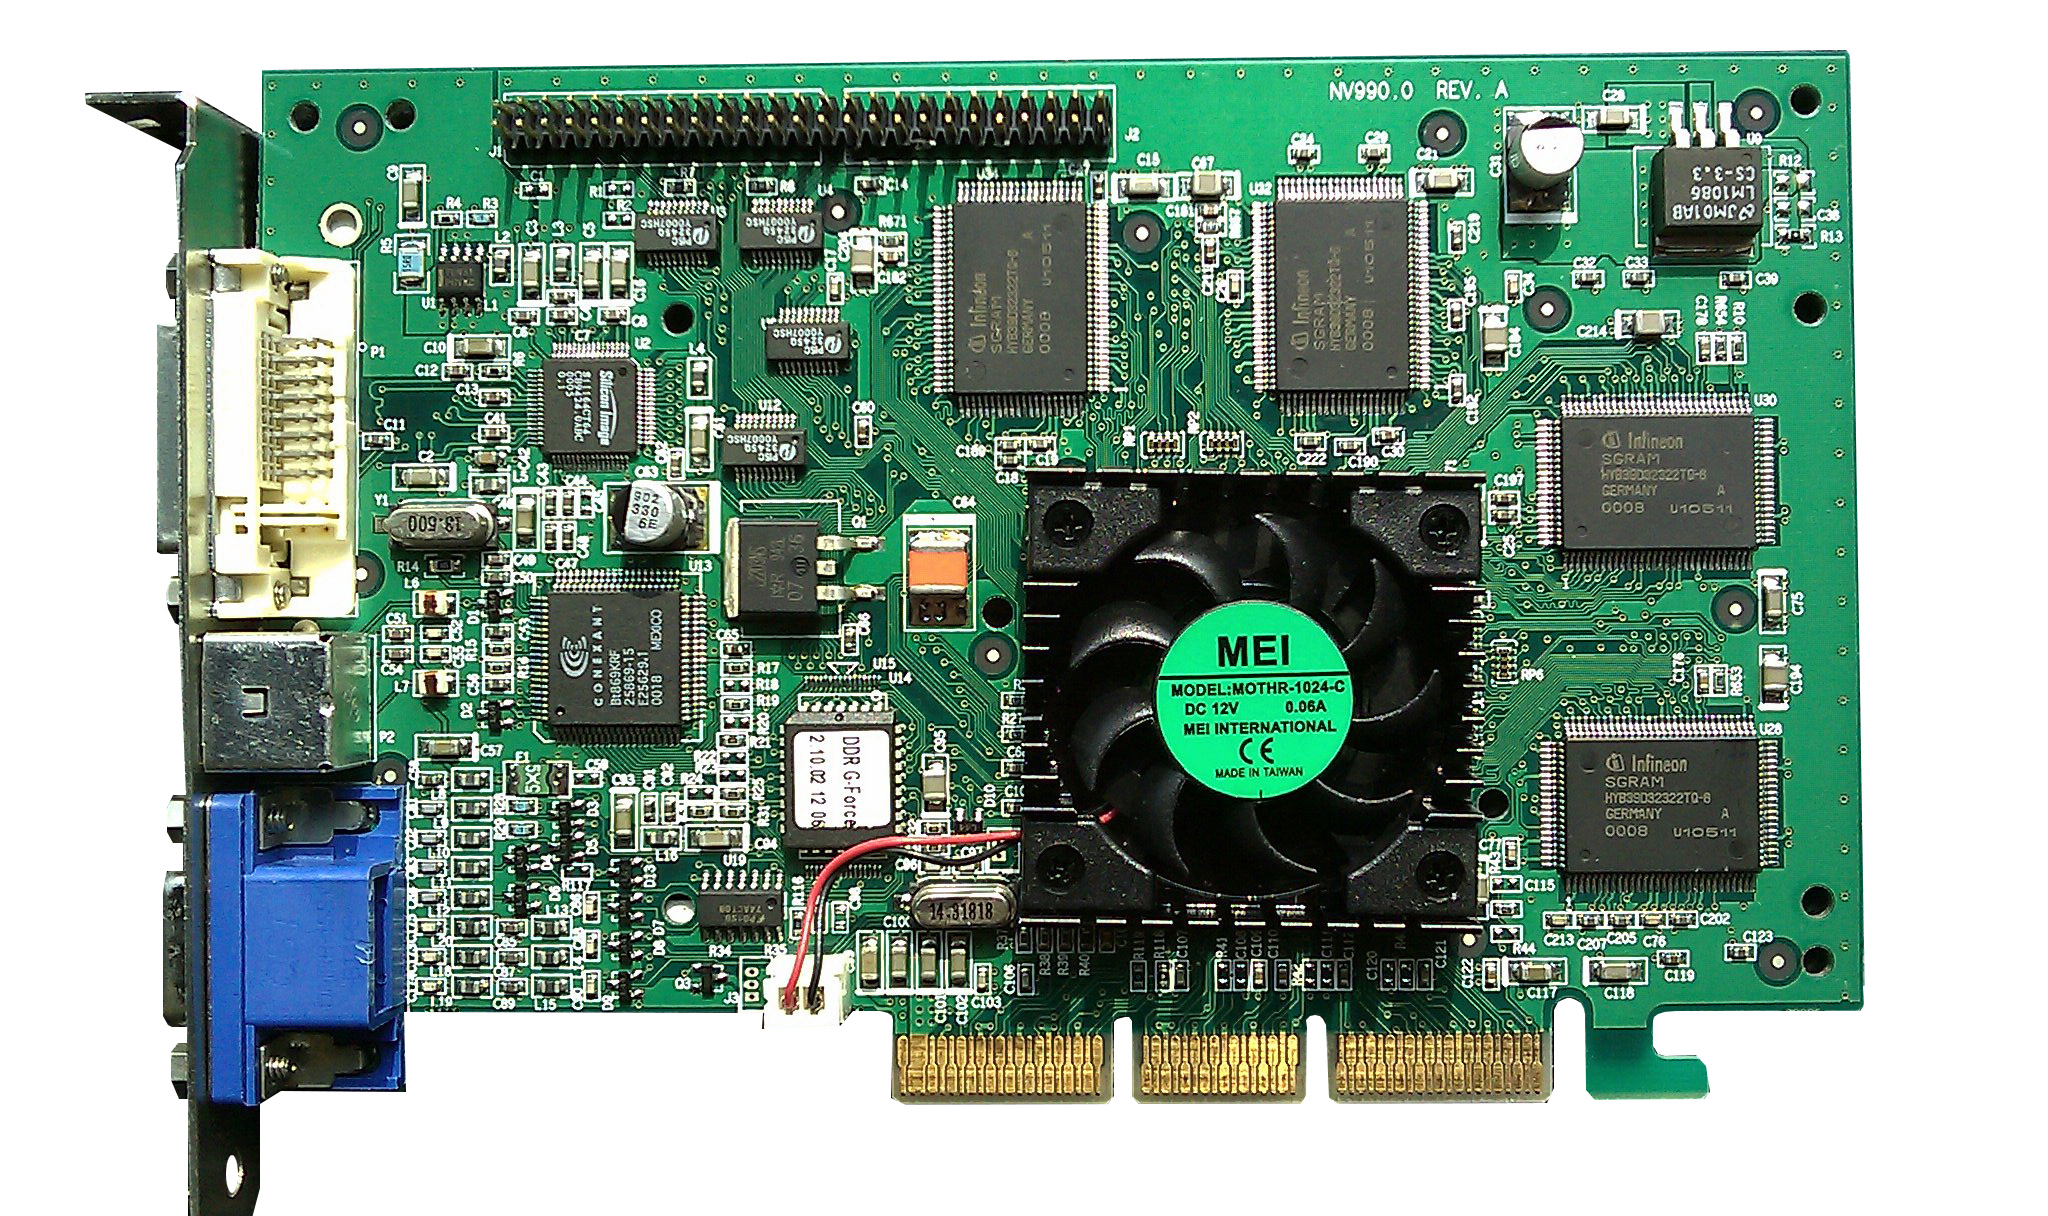
\includegraphics[width=\linewidth]{figuras/fig-a}}
		}{
		    \caption{GeForce 256} \label{fig:1a}
		}
		\nocite{figura4a}
        \end{subfigure}%
        
        \begin{subfigure}{0.30\textwidth}
        \UNIFORfig{}{
			\fbox{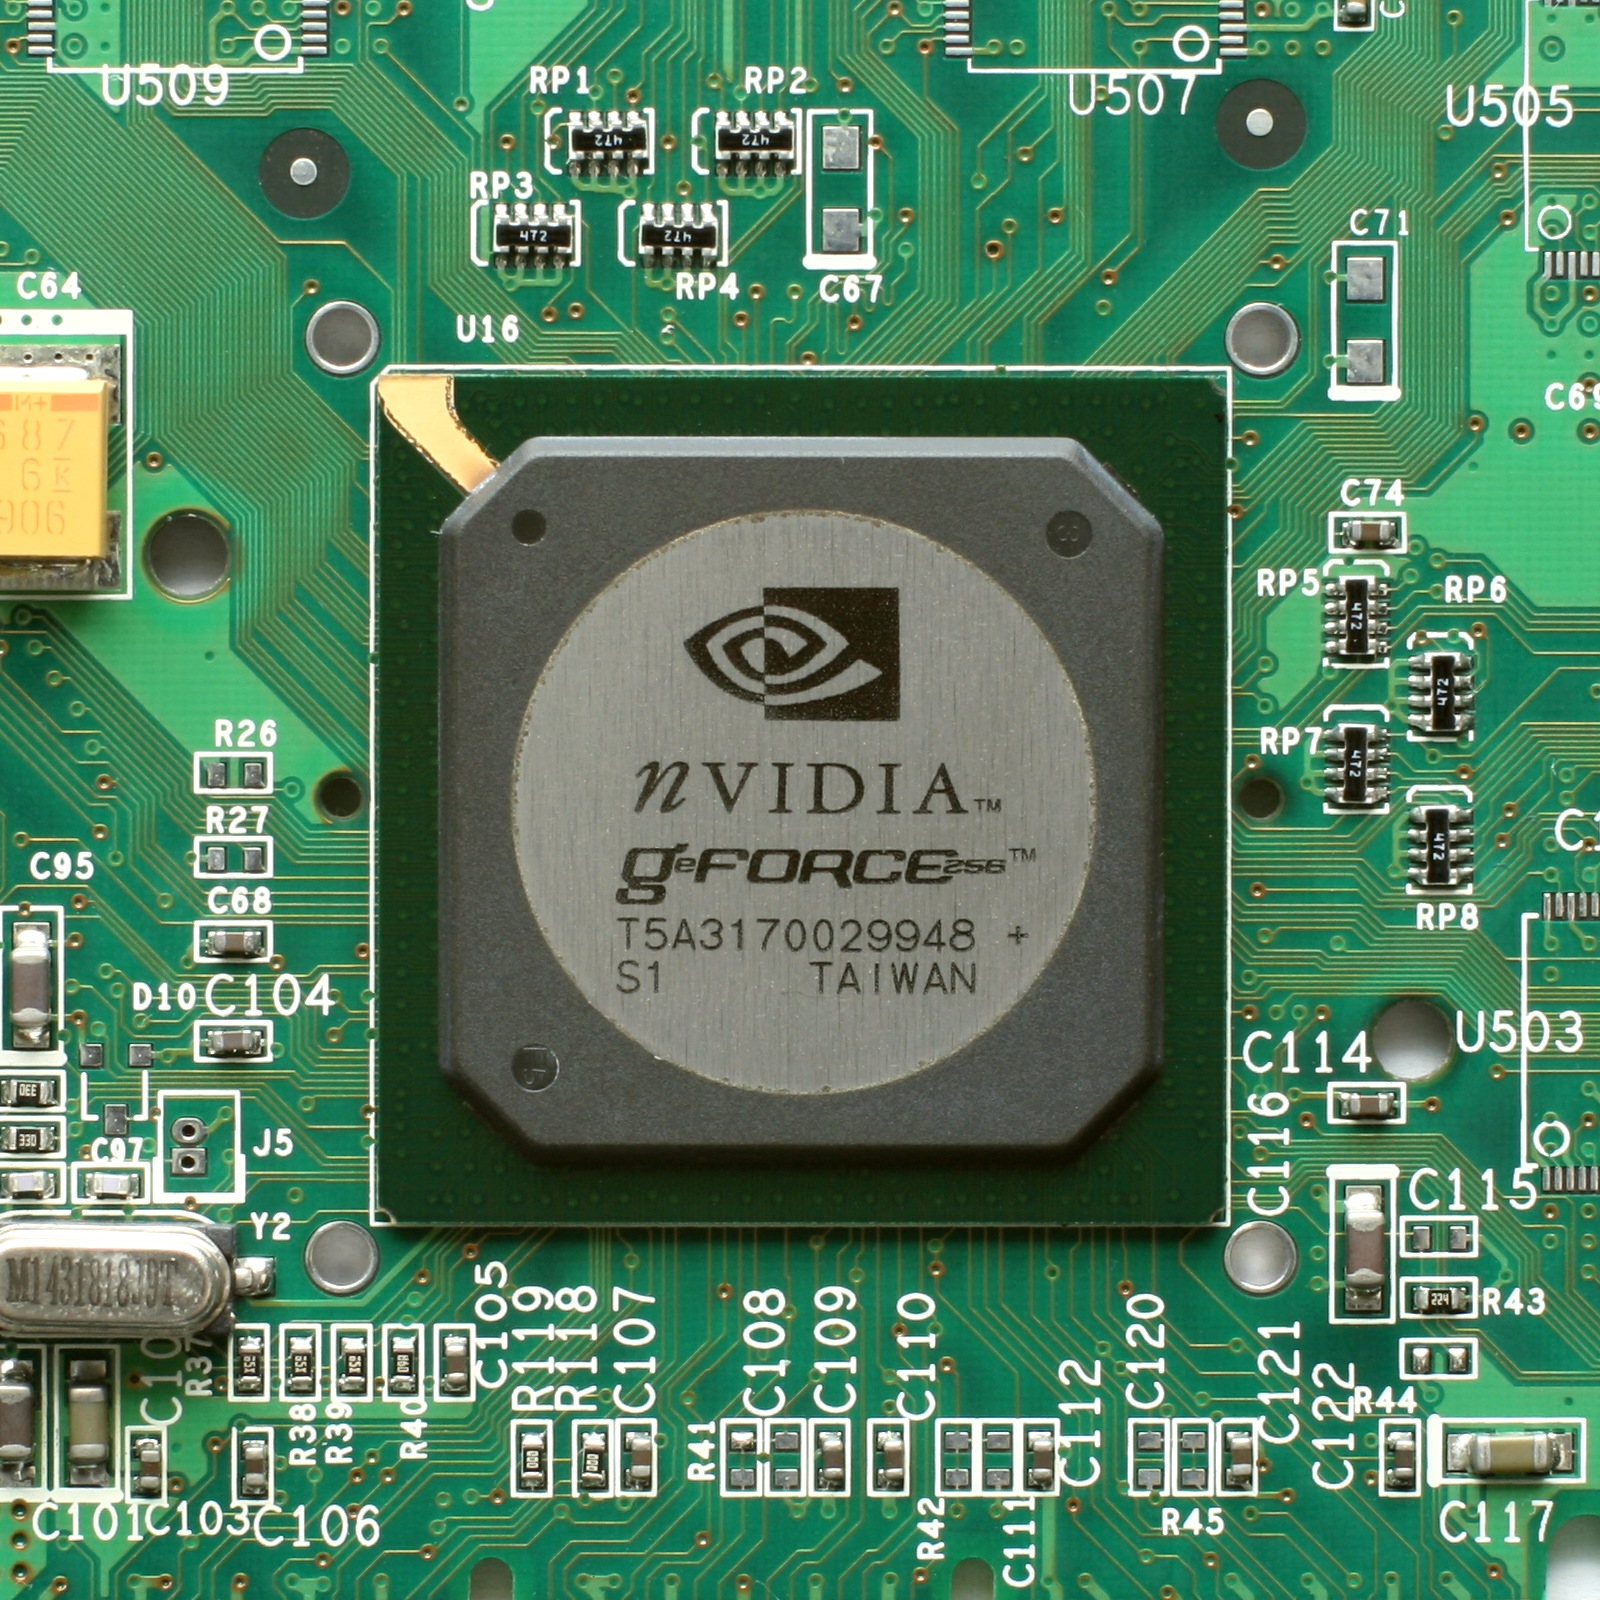
\includegraphics[width=\linewidth]{figuras/fig-b}}
		}{
		    \caption{GPU da GeForce 256} \label{fig:1b}
		}
		\nocite{figura4b}
        \end{subfigure}
		{
			\Fonte{https://upload.wikimedia.org/wikipedia/commons}
		}
	\end{figure}
	
Até então shaders eram bem vistos e utilizados por melhorar a performance eliminando carga de trabalho excessiva da \acrshort{CPU}, porém sua programação era difícil uma vez que a sintaxe utilizada era semelhante à programação em Assembly. Percebendo esse problema, a Microsoft lançou a versão 9.0 do Direct3D que trazia consigo a implementação da HLSL (\acrlong{HLSL}) que como o nome sugere permitia a programação de shaders em alto nível e possuia uma sintaxe bastante parecida com C. Enquanto isso, OpenGL também trouxe a sua própria linguagem de alto nível chamada GLSL (\acrlong{GLSL}) para competir no mercado (LUTEN, 2014)\nocite{openGLBook}. 

\subsection{Como o OpenGL funciona}
\label{sec:como-opengl-funciona}

Grosso modo, a API do OpenGL desenha gráficos em uma memória especializada em quadros de imagem (frame buffer) e os lê novamente quando precisa. O seu design único oferece suporte tanto a geometrias 3D quanto a imagens simples. O modelo de funcionamento dessa API pode ser descrito como cliente-servidor, pois a aplicação (cliente) faz solicitações por meio de comandos que são interpretados e processados pela implementação OpenGL (servidor) \cite{GLSLBook}. Aqui cabe destacar que a sincronia entre cliente e servidor e suas informações/dados não ocorre quando um comando é executado mas sim quando ele é emitido.

Os comandos são sempre processados na ordem em que são recebidos pelo servidor (execução fora de ordem não é permitida). Os dados passados para um comando OpenGL são então interpretados e copiados em memória caso seja necessário e as modificações subsequentes feitas pela aplicação não surtem efeito nos dados que estão armazenados internamente pelo OpenGL. Esses procedimentos são uma forma de garantir que um primitivo --- segundo Abdala (2019)\nocite{abdala}, uma representação discreta em grade de um elemento geométrico fundamental, e.g. ponto, linha, círculo, etc. --- seja desenhado apenas se o primitivo anterior houver sido completamente desenhado \cite{GLSLBook}.

OpenGL foi projetada para atuar como uma máquina de estados composta de parametros que definem o comportamento da pipeline de renderização e da forma que as primitivas são transformadas em pixels na tela. O estado é composto por uma estrutura de dados chamada contexto gráfico que é gerenciada pelo sistema de janelas do SO (\acrlong{SO}). O principio básico de funcionamento dessa API é transformar dados vindos de uma aplicação em algo visível na tela, esse processo é chamado de renderização e normalmente é acelerado por um hardware com design específico chamado de acelerador gráfico, entretanto suas operações podem ser parcial ou totalmente implementadas por software executado pela CPU. Aceleradores gráficos tipicamente possuem região de memória delimitada para manutenção do conteúdo exibido na tela, sendo que cada pixel é representado por uma quantidade de bytes na memória; uma tela em escala de cinza, por exemplo, pode fazer uso de um byte para representar a tonalidade de cinza de cada pixel \cite{GLSLBook}.

Essa região conhecida como memória de exibição é escaneada "x" vezes por segundo para eliminar a cintilação. Há ainda uma região específica para manipular dados que não são visíveis na tela chamada de memoria de não exibição. O responsável pela alocação de memória é o próprio sistema operacional que suporta o OpenGL. Em um sistema de janelas, a janela que corresponde a região da memória gráfica que é modificada durante a renderização é chamada de frame buffer. Já em um cenário sem janelas (i.e. tela cheia) o frame buffer corresponde a toda a tela \cite{GLSLBook}.

Para que uma janela consiga suportar a renderização ela precisa de uma combinação de alguns elementos: até quatro buffers para as cores, um buffer de profundidade (Figura 5), um \textit{stencil buffer} (Figura 6), um buffer de acumulação, um \textit{multisample buffer} e um ou mais buffers auxiliares. A maioria dos hardwares suporta o carregamento duplo, técnica que faz uso de um buffer frontal e um buffer posterior para que o processo de renderização seja realizado em plano de fundo e então quando terminar seu conteúdo é trocado com o do buffer frontal para exibir o resultado final e iniciar a nova renderização. Isso ajuda a conseguir animações suaves à taxas interativas \cite{GLSLBook}.

    \begin{figure}[h!]
		\centering
		\Caption{\label{fig:exemplo-6} O buffer de profundidade é mostrado em tons de cinza sendo que objetos próximos ficam com tonalidade mais escura enquanto objetos distantes assumem uma tonalidade mais clara.}	
		\UNIFORfig{}{
			\fbox{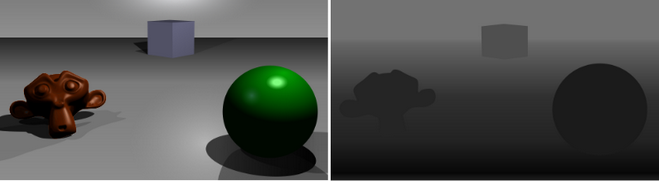
\includegraphics[width=15cm]{figuras/figura-6}}
		}{
			\Fonte{https://larranaga.github.io/Blog/imagenes/z-buffer.png}
		}
	\end{figure}
	\nocite{dptbuf}
	
No caso do suporte a visualização 3D estéreo, mais dois buffers serão utilizados em conjunto com os dois citados anteriormente para criar uma combinação com quatro buffers de cor que são divididos para cada olho. Se um objeto 3D precisa ser desenhado com remoção de superfície encoberta, o buffer de profundidade entra em ação comparando o valor da profundidade de cada pixel dos objetos em cena para determinar qual será visível ou obscurecido. E há ainda a opção do uso de um \textit{stencil buffer} para aplicar operações complexas utilizando máscaras com o objetivo de determinar onde cada pixel deve ser atualizado ou não \cite{GLSLBook}.

    \begin{figure}[h!]
		\centering
		\Caption{\label{fig:exemplo-7} O stencil buffer permite a customização da forma como objetos 3D são renderizados.}	
		\UNIFORfig{}{
			\fbox{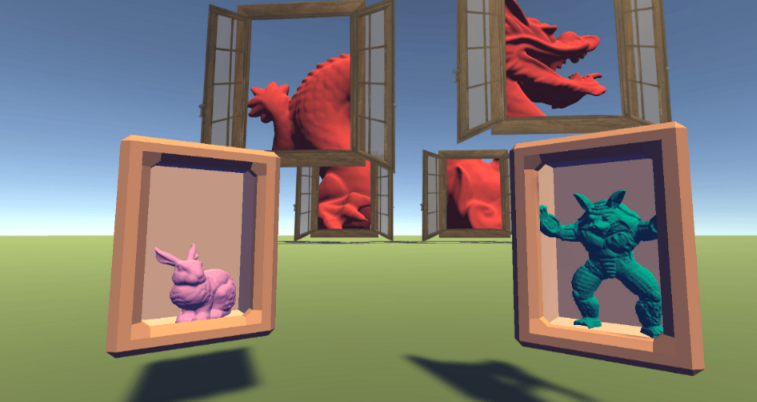
\includegraphics[width=15cm]{figuras/figura-7}}
		}{
			\Fonte{https://www.ronja-tutorials.com/assets/images/posts/022/Result.gif}
		}
	\end{figure}
	\nocite{stcbuf}

O buffer de acumulação é capaz de reproduzir efeitos complexos como suavização em tela cheia de alta qualidade, profundidade de campo e desfoque de movimento. Ele funciona como um buffer de cor, porém com maior precisão, capaz de acumular imagens para produzir uma úncia imagem composta. Seguindo essa linha, o \textit{multisample buffer} é capaz de produzir várias amostras da renderização para realizar suavização sem precisar renderizar a cena mais de uma vez \cite{GLSLBook}. Por último, os buffers auxiliares (mais de um pode ser utilizado) servem para guardar dados genéricos.

\subsubsection{Pipeline gráfica do OpenGL}
\label{sec:pipeline-opengl}

Para que a máquina de estados do OpenGL possa operar corretamente, foi definida uma ordem específica em que as operações envolvidas no processo de renderização precisam ser realizadas, essa padronização é chamada de \textit{pipeline} gráfica \cite{GLSLBook} e pode ser vista na Figura 7. Todos os dados necessários para desenhar a geometria estão contidos em espaço em memória e podem ser lidos pelo OpenGL de três maneiras diferentes. 

A primeira seria enviar um vértice de cada vez utilizando alguns comandos intermitentes para manipular atributos dos vértices. A segunda seria utilizar matrizes de vértices, o que oferece melhor performance devido a forma de organização dos dados, pois são utilizados ponteiros e mais dados podem ser processados de uma vez. Esses dois casos citados acima fazem uso do modo imediato pois as primitivas são renderizadas assim que são especificadas \cite{GLSLBook}. 

O terceiro modo seria utilizar algum dos dois procedimentos citados acima implementando uma lista de exibição, que é uma estrutura de dados que guarda comandos para execução futura. Algumas vantagens desse método no que diz respeito a performance seria a possibilidade de otimizar os comandos contidos na lista, ou ainda guardar os comandos na memória do acelerador gráfico para uma melhor performance de desenho \cite{GLSLBook}. 

	\begin{figure}[h!]
		\centering
		\Caption{\label{fig:pipeline} Pipeline gráfico do OpenGL.}	
		\UNIFORfig{}{
			\fbox{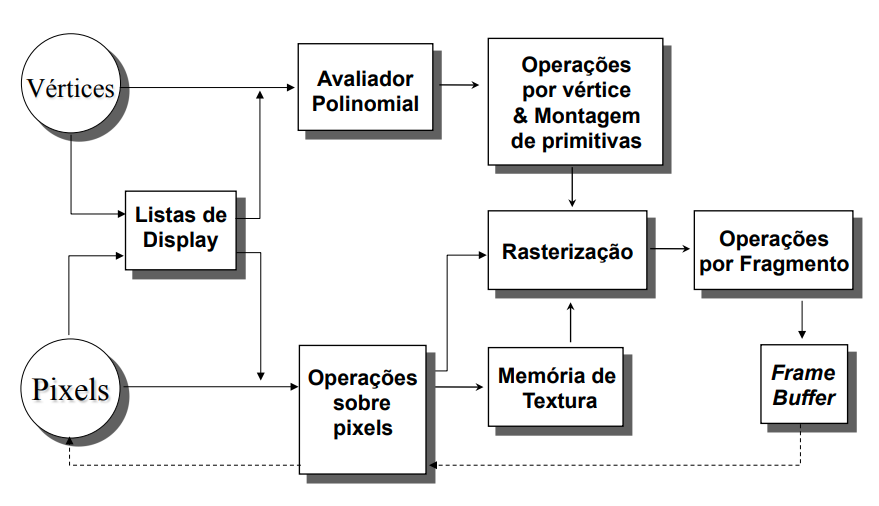
\includegraphics[width=15cm]{figuras/pipeline.png}}
		}{
			\Fonte{\url{http://www.ic.uff.br/~anselmo/cursos/CGI/slidesGrad/CG_aula4(introducaoaOpenGL).pdf}}
		}
	\end{figure}
	\nocite{pipeline}
	
Como todas as primitivas geométricas podem ser descritas por vértices, as curvas e as superfícies podem ser descritas pelas funções polinomiais chamadas funções base. A função do avaliador polinomial nesse caso é derivar os vértices para conseguir representar superfícies e curvas. Isso é feito através do método de mapeamento polinomial, que produz as normais da superfície, as coordenadas da textura, as cores, e valores de coordenadas espaciais dos pontos de controle (VIEIRA, 2017)\nocite{pipelnRef}.

A próxima etapa é o estágio das operações por vértice que converte os vértices em primitivas. Alguns dados do vértice são transformados em matrizes de pontos flutuantes. Nesta etapa ocorre a projeção de coordenadas do espaço do mundo para o espaço da tela. Inclui algumas etapas como geração e transformação de coordenadas de textura, e também cálculos de luz para produção dos valores de cor (VIEIRA, 2017). Por isso é normal que essa etapa exija mais recursos computacionais. 

Logo em seguida ocorre a montagem das primitivas por meio do \textit{clipping} (eliminação de parte da geometria desnecessária para a renderização), que é um processo onde se a primitiva está totalmente dentro do plano de visualização ela é repassada para o devido processamento. Caso ela esteja totalmente fora do plano de visualização ela é rejeitada e não é processada. Se a primitiva estiver parcialmente visível no plano, ela é dividida para que somente a porção visível siga para processamento.

Outra operação que ocorre nesse estágio é a projeção das coordenadas da perspectiva para coordenadas da janela. Além disso, há ainda uma etapa opcional de \textit{culling} onde os polígonos são testados para saber se será preciso descartar faces posteriores, anteriores ou ambas \cite{GLSLBook}. Paralelamente a esse processo, os dados de pixels contidos em uma matriz na memória do sistema são empacotados e escalados, inclinados e processados por um mapa de pixels. Os resultados, que serão então empacotados em um formato apropriado e retornados a uma matriz de memória do sistema, podem ser escritos na memória da textura ou emitidos à uma etapa de rasterização.

Rasterização é a etapa de conversão de dados tanto geométricos como de pixel em fragmentos. Cada quadrado do fragmento corresponde a um pixel no \textit{frame buffer}, sendo que os valores da cor e da profundidade são atribuídos para cada um. Ao final são executadas mais algumas operações antes de armazenar os valores no \textit{frame buffer} como: \textit{texturing}, onde um elemento da textura é gerado e aplicado da memória da textura para cada fragmento; cálculos de névoa; testes de profundidade, transparência e remoção de faces ocultas (VIEIRA, 2017). Apesar dessa etapa possuir muitos processos, as operações são relativamente simples e podem ser executadas eficientemente para milhões de pixels por segundo com o hardware disponível atualmente.

Em relação a etapa de texturização, uma das mais complexas, é interessante destacar que a API tem capacidade de trabalhar com quatro tipos de texturas. Texturas de uma dimensão (vetor de pixels), texturas 2D (matriz $ mxn $ de pixels), texturas 3D (matriz com uma dimensão a mais para guardar informações adicionais e.g. profundidade), e mapas cúbicos (normalmente usado para simular reflexões de ambiente). A API também fornece métodos para trabalhar com formatos de imagem compactados, esses usam significativamente menos memória e melhoram a performance \cite{GLSLBook}.

É importante destacar que a API também fornece a possibilidade de utilizar texturas do tipo \textit{mipmap} --- várias representações da mesma imagem, porém cada uma tem metade da resolução da anterior --- em conjunto com o parâmetro de nível de detalhe que será detalhado mais adiante, mas que de forma simplificada permite a otimização do processo de renderização de objetos que estão distantes da câmera. 

\subsubsection{Matrizes de transformação de coordenadas}
\label{sec:matrizes-transformacao-coordenadas}

Esse é um tópico mais complexo, mas que também é importante para entender como a pipeline gráfica do OpenGL transforma descrições de objetos tridimensionais em imagens 2D que são exibidas na tela (Figura \ref{fig:spaces}). Algo semelhante a como uma câmera pode ser usada para criar uma representação em imagem de algo no mundo real. Entretanto nesse caso o primeiro passo consiste em pegar as informações do modelo do objeto 3D, como posição dos vértices e normais da superfície, para interpretá-las como coordenadas do espaço do objeto \cite{GLSLBook}. 

	\begin{figure}[htp]
		\centering
		\Caption{\label{fig:spaces} Processo de transformação entre os sistemas de coordenadas e seus espaços.}	
		\UNIFORfig{}{
			\fbox{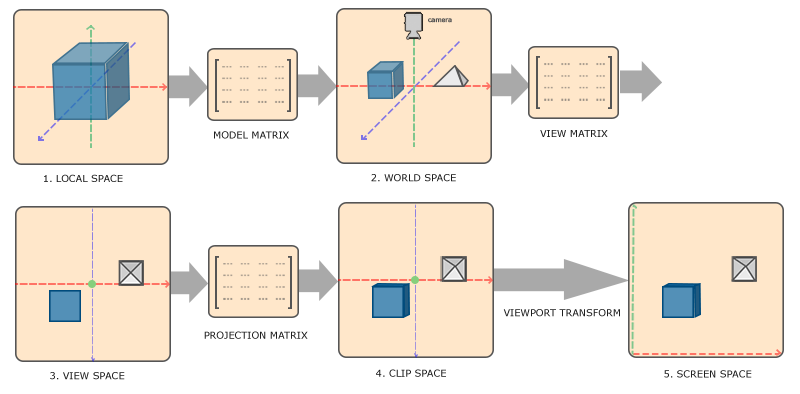
\includegraphics[width=12cm]{figuras/spaces.png}}
		}{
			\Fonte{\url{https://learnopengl.com/img/getting-started/coordinate_systems.png}}
		}
	\end{figure}
	\nocite{spaces}

Como cada objeto tem suas próprias características é necessário definir um sistema de coordenadas uniforme para que seja possível usar vários objetos em uma única cena. Para isso é utilizado o sistema de coordenadas global, e aqui a API vai um passo além e realiza mais uma conversão para o sistema de coordenadas de olho levando em consideração a posição da câmera na cena, seu ponto focal (para onde a câmera está olhando) e o vetor de direção para cima (e.g. a orientação da câmera) \cite{GLSLBook}. 

	\begin{equation}
		\begin{bmatrix}
			x_{olho} \\
			y_{olho} \\
			z_{olho} \\
			w_{olho} \\
		\end{bmatrix}
		=
		M_{modelView} \cdot
		\begin{bmatrix}
			x_{obj} \\
			y_{obj} \\
			z_{obj} \\
			w_{obj} \\
		\end{bmatrix}
	\end{equation}

Na equação 2.1, a matriz \textit{modelView} é uma multiplicação das matrizes de conversão de coordenadas de espaço de objeto para espaço global e de espaço global para espaço de olho. O cálculo das normais é semelhante, a diferença é que é utilizada a matriz transposta da inversa da matriz \textit{modelView} para multiplicar um vetor de normais. Como é possível ver na Figura \ref{fig:worldview} os três elementos mais à direita ($ m_{12} $, $ m_{13} $, $ m_{14} $) são para transformação de translação. O $ m_{15} $ é uma coordenada homogênea (Apêndice --- A) usada para transformação para o espaço de projeção. Os três conjunto de elementos ($ m_{0} $, $ m_{1} $, $ m_{2} $), ($ m_{4} $, $ m_{5} $, $ m_{6} $) e ($ m_{8} $, $ m_{9} $, $ m_{10} $) são usados para rotação e escala e representam os três eixos ortogonais x, y e z (AHN, 2013)\nocite{openglOnline}.

	\begin{figure}[h!]
		\centering
		\Caption{\label{fig:worldview} Conteúdo das quatro colunas da matriz \textit{modelView}.}	
		\UNIFORfig{}{
			\fbox{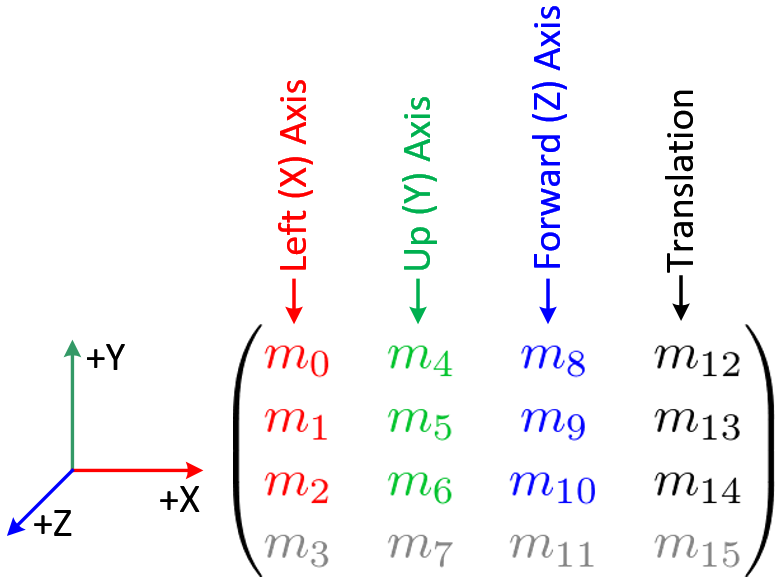
\includegraphics[width=7cm]{figuras/modelView.png}}
		}{
			\Fonte{\url{http://www.songho.ca/opengl/gl_transform.html}}
		}
	\end{figure}

Após essa conversão, as coordenadas obtidas são multiplicadas pela matriz de projeção para definir como os vértices serão projetados na tela, os valores dessa matriz dependem se modo de projeção utilizado é em perspectiva ou ortográfico (Figura \ref{fig:frustum}) e são mostrados nas equações \ref{eq-persp} e \ref{eq-ortho} respectivamente. 

	\begin{equation} \label{eq-persp}
		\resizebox{.35\hsize}{!}{$ M_{persp}
		=
		\begin{bmatrix}
			\cfrac{2n}{r-l} & 0 & \cfrac{r+l}{r-l} & 0 \\
			0 & \cfrac{2n}{t-b} & \cfrac{t+b}{t-b} & 0 \\
			0 & 0 & \cfrac{-(f+n)}{f-n} & \cfrac{-2fn}{f-n}\\
			0 & 0 & -1 & 0 \\
		\end{bmatrix} $}
	\end{equation}
	\begin{equation} \label{eq-ortho}
		\resizebox{.35\hsize}{!}{$ M_{orto}
		=
		\begin{bmatrix}
			\cfrac{2}{r-l} & 0 & 0 & -\cfrac{r+l}{r-l} \\
			0 & \cfrac{2}{t-b} & 0 & -\cfrac{t+b}{t-b} \\
			0 & 0 & \cfrac{-2}{f-n} & -\cfrac{f+n}{f-n}\\
			0 & 0 & 0 & 1 \\
		\end{bmatrix} $}
	\end{equation}

Os valores obtidos nessa operação são normalizados em uma região cúbica definida pelos pontos (-1, -1, -1) e (1, 1, 1) para espaço de coordenadas de dispositivo normalizado, isso significa que os valores passam a ser algum valor entre -1 e 1. Essa etapa é necessária para qua a área de visualização seja apropriadamente mapeada em uma janela de exibição de tamanho arbitrário. Por último, as coordenadas são convertidas para o sistema de coordenadas de tela. A partir desse ponto elas continuam para o processo de rasterização da pipeline do OpenGL (AHN, 2013)\nocite{openglOnline}. 
	\begin{figure}[hbp]
		\centering
        \Caption{\label{fig:frustum} Modos de projeção de câmera. As letras correspondem a \textit{left, right, bottom, top, near e far}.}
        \begin{subfigure}{0.45\textwidth}
        \UNIFORfig{}{
			\fbox{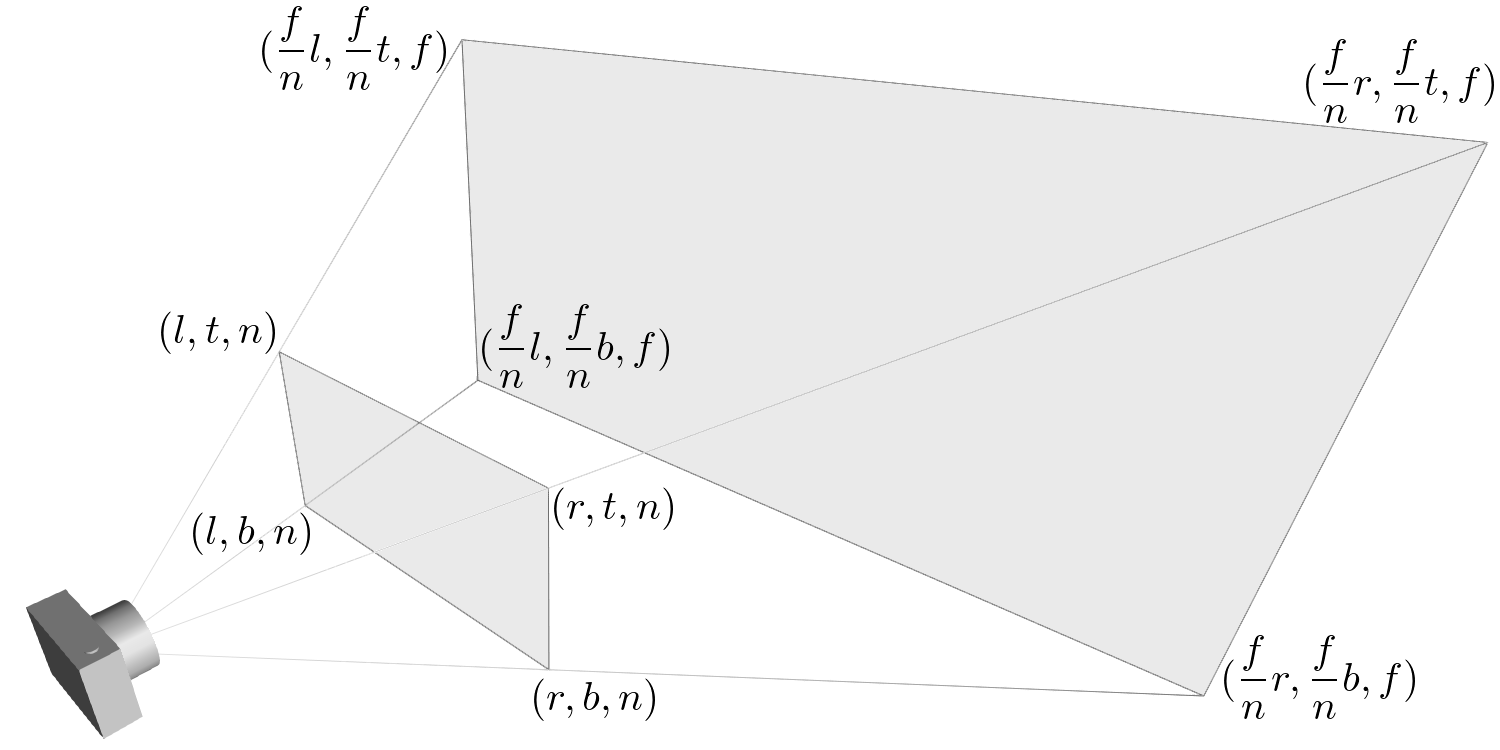
\includegraphics[width=\linewidth]{figuras/persp.png}}
		}{
		    \caption{\Gls{view-frustum} em perspectiva}
		}
        \end{subfigure}
		\hfill
        \begin{subfigure}{0.47\textwidth}
        \UNIFORfig{}{
			\fbox{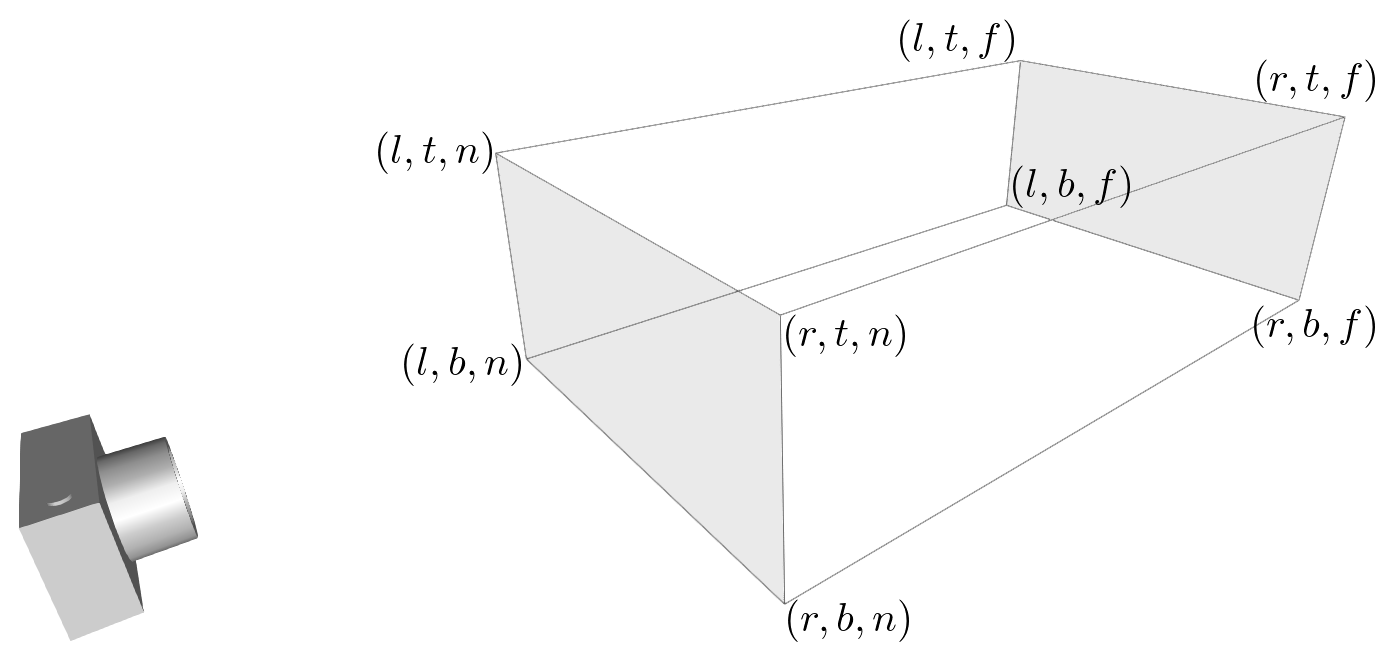
\includegraphics[width=\linewidth]{figuras/ortho.png}}
		}{
		    \caption{\Gls{view-frustum} ortográfico}
		}
        \end{subfigure}
		{
			\Fonte{\url{http://www.songho.ca/opengl/gl_transform.html}}
		}
	\end{figure}

\subsection{OpenGL Shading Language}
\label{sec:glsl}

Devido à necessidade crescente de substituir funcionalidades fixas por programabilidade em áreas que ficavam cada vez mais complexas, como processamento de vértices e fragmentos, foi desenvolvida uma solução que adicionou estágios programáveis para resolver esse problema. Essa solução foi a introdução da linguagem de sombreamento \acrshort{GLSL}, feita para ser executada nos dois processadores programáveis existentes no OpenGL: o processador de vértices e o processador de fragmentos (portanto os respectivos nomes \textit{vertex shader} e \textit{fragment shader}) \cite{GLSLBook}. 

Um shader pode então ser definido como um código escrito em uma linguagem de sombreamento (HLSL, GLSL, RSL e etc) com o propósito de ser executado por um dos processadores programáveis do OpenGL. Um programa de shader é então um conjunto de shaders compilados executáveis \cite{GLSLBook}. A Figura \ref{fig:outline} mostra a implementação do código-fonte \ref{cf:outline} para criar um efeito de linha de contorno em volta de um objeto 3D utilizando a linguagem GLSL.

	\begin{figure}[h!]
		\centering
		\Caption{\label{fig:outline} Demonstração de um shader simples de linha contorno.}	
		\UNIFORfig{}{
			\fbox{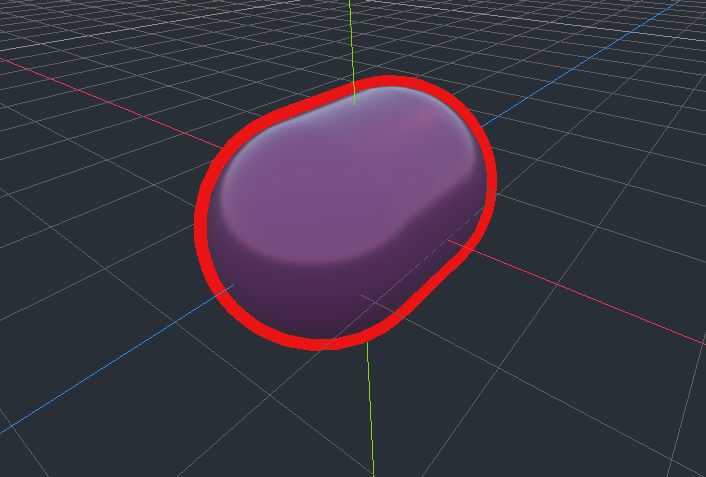
\includegraphics[width=8cm]{figuras/outline.png}}
		}{
			\Fonte{Elaborado pelo autor}
		}
	\end{figure}

A linguagem de sombreamento GLSL faz uso de uma sintaxe bastante similar a linguagem de programação C. Seus tipos incluem vetores e matrizes por serem estruturas fundamentais para cálculos matemáticos com operações para gráficos 3D. O uso de números de ponto flutuante (\textit{float}) também é fundamental para conseguir altos níveis de precisão a troco de performance, por isso é possível especificar o nível de precisão desejado ao utilizá-los. Além disso ela oferece suporte a laços, chamadas a sub-rotinas, expressões condicionais e conta com funções embutidas próprias para o desenvolvimento de shaders \cite{GLSLBook}. 

Essa linguagem possibilitou aos desenvolvedores implementar um conjunto de diferentes técnicas para conseguir obter uma variedade enorme de efeitos visuais; não somente isso mas o fato de que essas técnicas são implementadas com aceleração via hardware pela GPU (com processamento paralelo) proporciona um aumento drástico de performance e libera carga da CPU para realizar outras tarefas \cite{GLSLBook}.

O processador de vértices é uma unidade programável que realiza operações nos valores de vértices recebidos e seus dados associados. Essas operações consistem em transformação de vértices, transformação e normalização das normais, geração e transformação das coordenadas de textura, iluminação e aplicação de cor. Shaders feitos para rodar nesse processador são chamados de shaders de vértice \cite{GLSLBook}. 

Variáveis de atributo (variável global somente leitura alterada por vértice) são utilizadas para passar valores da aplicação para o processador de vértices. Já as variáveis uniformes (variável global somente leitura alterada por primitiva) são utilizadas para passar dados tanto para o processador de vértices como de fragmentos. Por último há as variáveis variantes cuja função é transportar informação do processador de vértices para o processador de fragmentos \cite{GLSLBook}.

O processador de vértices atua em um vértice por vez e uma implementação pode ter múltiplos processadores operando em paralelo (o mesmo vale para o processador de fragmentos). Logo, o shader de vértice é executado uma vez para cada vértice, sendo que há uma possibilidade de perda de performance caso um shader de vértice precise calcular mais variáveis variantes do que o que é necessário pelo shader de fragmentos. Por outro lado, o processador de fragmentos é responsável por realizar algumas operações como interpolação de valores, acesso e aplicação de texturas, névoa e soma de cor \cite{GLSLBook}. 

Cabe ressaltar que, em termos de performance, normalmente os desenvolvedores preferem utilizar um shader de vértice mais genérico em conjunto com um shader de fragmento, pois assim é possível utilizar apenas um subconjunto das variáveis contidas no shader de vértice e ainda sim reduzir tempo e custos de desenvolvimento e manutenção para uma grande quantidade de shaders \cite{GLSLBook}.

\subsection{Direct3D (HLSL) \textit{versus} OpenGL (GLSL)}
\label{sec:direct-versus-opengl}

Direct3D é uma API para desenvolvimento de aplicações gráficas nativas para plataformas proprietárias da Microsoft. Ela evoluiu muito durante os anos anos 90 e superou a OpenGL. Conceitualmente, a pipeline gráfica de ambas APIs são bem semelhantes, mas uma diferença importante se dá em termos de design de gerenciamento dos estágios de shaders, onde OpenGL faz uso de um objeto (programa de shader) que contém múltiplos shaders enquanto que Direct3D expõe um contexto de renderização diretamente para a criação de shaders. Quanto às linguagens (GLSL e HLSL), são muito parecidas e os desenvolvedores conseguem transcrever instruções facilmente de uma para a outra (MICROSOFT, 2020)\nocite{Direct3D}.

Considerando a pouca diferença em capacidade de renderização existente entre essas duas interfaces, a escolha sobre qual usar depende muito da plataforma alvo de desenvolvimento. Direct3D é específica para plataformas da Microsoft e é amplamente suportada por fornecedores de hardware gráfico, especialmente em computadores desktop. OpenGL é open source e possui bastante aceitação no espaço de desenvolvimento mobile, principalmente devido ao desenvolvimento da OpenGL ES --- uma subseção do OpenGL projetada especialmente para sistemas embarcados como smartphones e consoles portáteis \cite{HLSLBook}.

\subsection{High-Level Shader Language}
\label{sec:hlsl}

A HLSL é uma linguagem de shader criada em 2002 (acompanhou o DirectX 9) e também assemelha-se à linguagem de programação C. Ao longo dos anos foram adicionadas melhorias como suporte a \textit{\Gls{multithread}}, adição de uma API específica para uso de GPGPU (\acrlong{GPGPU}) e o suporte a tesselação. Na Figura \ref{fig:outlineHLSL} abaixo é mostrada a implementação um shader de contorno (ver código-fonte \ref{cf:outlineHLSL}) similar ao anterior para demonstrar algumas diferenças e semelhanças entre as duas linguagens.

	\begin{figure}[h!]
		\centering
		\Caption{\label{fig:outlineHLSL} O mesmo resultado de contorno obtido com HLSL.}	
		\UNIFORfig{}{
			\fbox{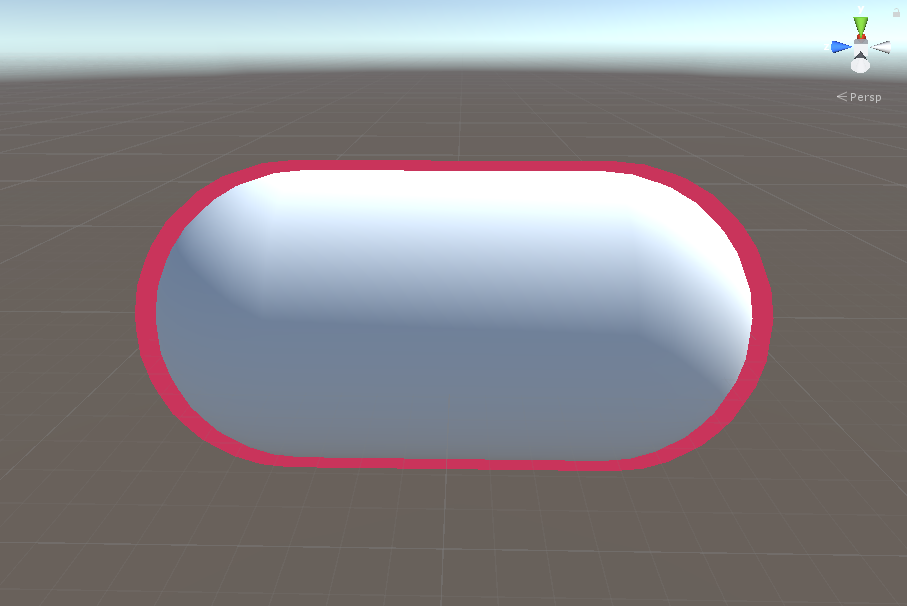
\includegraphics[width=7cm]{figuras/outlineUnity.PNG}}
		}{
			\Fonte{Elaborado pelo autor}
		}
	\end{figure}

Uma GPU de propósito geral é uma unidade de processamento gráfico (GPU) que realiza cálculos genéricos que normalmente seriam feitos pela CPU. São utilizadas para realizar tarefas custosas como cálculos de física, criptografia e computações científicas, pois é possível tirar proveito do paralelismo disponível nas placas gráficas. Da mesma forma que um núcleo pode ser utilizado para renderizar múltiplos pixels simultaneamente, ele também é capaz de processar múltiplos fluxos de dados ao mesmo tempo (TECHTARGET, 2015)\nocite{GPGPU}.

Tesselação é mais um processo na pipeline gráfica responsável por adicionar detalhes a objetos diretamente pela GPU. De maneira geral, mais detalhes geometricos (mais vértices), resultam em uma renderização "mais bonita". Seu modo de funcionamento consiste em subdividir um objeto dinamicamente e sem o custo adicional de reprocessamento de geometria. Isso permite um sistema de nível de detalhe dinâmico e menos utilização do barramento de gráficos, o que melhora a performance \cite{HLSLBook}.

	\begin{figure}[h!]
		\centering
		\Caption{\label{fig:tess} Diferentes níveis de tesselação aplicados em uma malha produzem aumento no número de vértices.}	
		\UNIFORfig{}{
			\fbox{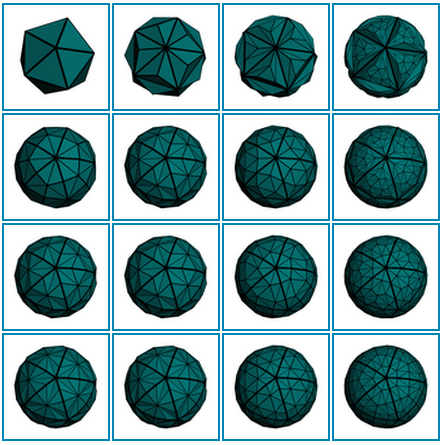
\includegraphics[width=7cm]{figuras/tess.png}}
		}{
			\Fonte{\url{https://upload.wikimedia.org/wikipedia/commons/f/fc/Tessellation_Level_Table.png}}
		}
	\end{figure}
	\nocite{tesselation}

\section{Aprofundando Conceitos Técnicos de Shaders}
\label{sec:aprofundando-conceitos-tecnicos-shaders}

% Caso for adicionar mais texto sobre %
% HLSL, adicionar nessa parte         %

Ao estudar computação gráfica a dúvida mais comum ao se deparar com certos termos utilizados é "o que é um shader". Essa palavra pode causar uma certa estranheza no início mas sua definição não é nenhum bicho de sete cabeças. Shaders são apenas pequenos programas (assim como um reprodutor de mídia ou uma calculadora de um computador) que são executados diretamente pela \acrshort{GPU} ao invés da \acrshort{CPU}. Isso permite a redução da carga de trabalho gráfico da \acrshort{CPU} pelo redirecionamento das tarefas para a \acrshort{GPU} que possui hardware especializado para isso (LUTEN, 2014)\nocite{openGLBook}.

	\begin{figure}[h!]
		\centering
		\Caption{\label{fig:exemplo-5} Demonstração de como é possível criar visuais únicos utilizando shaders.}	
		\UNIFORfig{}{
			\fbox{
\includegraphics[width=10cm]{figuras/figura-5}}
		}{
			\Fonte{Adaptado de \url{https://www.youtube.com/watch?time_continue=2&v=F0CWzpYY68A&feature=emb_logo}}
		}
	\end{figure}
	\nocite{figura5}

Tecnicamente falando, um shader contém um conjunto de instruções que são executadas concorrentemente para cada pixel desenhado na tela. Essa forma de operação abre um leque de possibilidades, onde é possível por exemplo atribuir um comportamento para cada pixel baseado na sua posição na tela. Em uma comparação com programação procedural, ele funcionaria como uma função que recebe uma posição e retorna uma cor, sendo que após a compilação seu tempo de execução é extremamente rápido (VIVO; LOWE, 2015)\nocite{bookOfShaders}.

Uma metáfora para ajudar a compreender a dimensão da complexidade do processamento de um shader seria imaginá-lo como um bloco de várias tarefas que passa por uma linha de produção industrial. As tarefas podem ser pequenas ou grandes e consequentemente podem demandar mais processamento e energia. No caso da CPU cada trabalho seguinte teria que esperar o término do atual para começar (VIVO; LOWE, 2015)\nocite{bookOfShaders}. É interessante ressaltar que hoje em dia existe a tecnologia de multiprocessamento, onde os computadores normalmente possuem grupos de quatro processadores que atuam em conjunto para realizar as tarefas.

Considerando uma tela com resolução de 800x600, significa que 480.000 pixels precisam ser processados a cada frame sendo que normalmente é utilizada uma taxa de 30 frames por segundo (\acrshort{FPS}), então será necessário fazer 14.400.000 cálculos por segundo. Isso explica o fato de video games e outras aplicações gráficas exigirem muito mais poder de processamento que outros programas. Seu conteúdo gráfico implica em inúmeras operações por cada pixel, pois cada pixel na tela precisa ser computado, e também em perspectivas e geometrias de jogos 3D (VIVO; LOWE, 2015)\nocite{bookOfShaders}.  

Esse cenário pode ser suficiente para sobrecarregar um microprocessador comum e fica pior quando leva-se em consideração as tecnologias que fazem uso seja de taxa de FPS maior, seja de resoluções maiores como 2K, e acima. Para resolver esse problema utiliza-se processamento paralelo. A GPU possui vários pequenos microprocessadores que funcionam concorrentemente, além disso ela possui funções matemáticas específicas aceleradas via hardware para realizar operações matriciais e trigonométricas rapidamente (VIVO; LOWE, 2015)\nocite{bookOfShaders}.


\subsection{Vertex Shader}

A vertex shader is a GPU program that is executed once per vertex that is assigned to, and a pixel shader is a GPU program that is executed once per pixel.
Vertex processing involves the operations that occur at each vertex, most notably transformation and lighting. Fragments are per-pixel data structures that are created by the rasterization of graphics primitives. A fragment contains all the data necessary to update a single location in the frame buffer. Fragment processing consists of the operations that occur on a per-fragment basis, most notably reading from texture memory and applying the texture value(s) at each fragment \cite{GLSLBook}.

\subsection{Fragment Shader}

\section{Godot}
\label{sec:unity}

\section{Unity}
\label{sec:unity}

\subsection{ShaderLab}
\label{sec:shaderlab}

\section{Unreal}
\label{sec:unity}

\subsection{Nós de material}
\label{sec:shaderlab}

\section{Otimização e performance}
\label{sec:otimizacao-performance}


Nunc ac pretium dui. Mauris aliquam dapibus nulla ac mattis. Aenean non tortor volutpat, varius lectus vitae, accumsan nibh. Cras pretium vestibulum enim, id ullamcorper tortor ultrices non. Integer sodales viverra faucibus. Curabitur at dui lacinia, rhoncus lacus at, blandit metus. Integer scelerisque non enim quis ornare.

\lipsum[13]

	\begin{table}[h!]	
		\centering
		\Caption{\label{tab:exemplo-3} Duis faucibus, enim quis tincidunt pellentesque, nisl leo varius nulla, vitae tempus dui mauris ac ante purus lorem}		
		\UNIFORtab{}{
			\begin{tabular}{cll}
				\toprule
				Ranking & Exon Coverage & Splice Site Support \\
				\midrule \midrule
				E1 & Complete coverage by a single transcript & Both splice sites\\
				E2 & Complete coverage by more than a single transcript & Both splice sites\\
				E3 & Partial coverage & Both splice sites\\
				E4 & Partial coverage & One splice site\\
				E5 & Complete or partial coverage & No splice sites\\
				E6 & No coverage & No splice sites\\
				\bottomrule
			\end{tabular}
		}{
		\Fonte{Elaborado pelo autor}
	}
	\end{table}

Duis faucibus, enim quis tincidunt pellentesque, nisl leo varius nulla, vitae tempus dui mauris ac ante. Quisque purus lorem, pharetra sit amet lobortis eu, vehicula vitae purus. Ut varius, erat nec vehicula elementum, risus est tempus justo, nec vulputate augue leo egestas metus.

\lipsum[14]

	\begin{table}[h!]	
		\centering
		\Caption{\label{tab:exemplo-5} Etiam molestie, nulla a egestas aliquet, velit augue congue metus}		
		\UNIFORtab{}{
			\begin{tabular}{ccll}
				\toprule
				Quisque & pharetra & tempus & vulputate \\
				\midrule \midrule
				E1 & Complete coverage by a single transcript & Both splice sites\\
				E2 & Complete coverage by more than a single transcript & Both splice sites\\
				E3 & Partial coverage & Both splice sites & Both \\
				E4 & Partial coverage & One splice site & Both \\
				E5 & Complete or partial coverage & No splice sites & Both\\
				E6 & No coverage & No splice sites\\
				\bottomrule
			\end{tabular}
		}{
		\Fonte{Elaborado pelo autor}
	}
	\end{table}
	
	%como usar as siglas e abreviações
	%\acrlong{MIT}
	\acrlong{MIT}

\begin{alineascomponto}
	\item Integer non lacinia magna. Aenean tempor lorem tellus, non sodales nisl commodo ut
	\item Proin mattis placerat risus sit amet laoreet. Praesent sapien arcu, maximus ac fringilla efficitur, vulputate faucibus sem. Donec aliquet velit eros, sit amet elementum dolor pharetra eget
	\item Integer eget mattis libero. Praesent ex velit, pulvinar at massa vel, fermentum dictum mauris. Ut feugiat accumsan augue, et ultrices ipsum euismod vitae
	\begin{subalineascomponto}
		\item Integer non lacinia magna. Aenean tempor lorem tellus, non sodales nisl commodo ut
		\item Proin mattis placerat risus sit amet laoreet.
	\end{subalineascomponto}
\end{alineascomponto}